\section{Convolutional Neural Networks}
\label{sec:cnn}

The multilayer networks of Section~\ref{sec:neural-networks} accept any input
vector, and that generality is exactly their weakness on images. An image is not
an arbitrary list of numbers: neighboring pixels belong together, and the same
pattern means the same thing wherever it appears. Convolutional neural networks
(ConvNets, CNNs) build these two facts into the architecture. Each unit looks
only at a small local patch, and the same weights are reused at every position.
The result is a network with far fewer parameters that learns much more from the
same amount of data.

This section first explains why fully connected networks are a poor fit for
images and which property a good image network should have. It then builds the
convolutional layer step by step in one dimension, where every quantity can be
drawn and computed by hand, and extends it with channels, receptive fields,
two-dimensional kernels, and down- and upsampling. A small experiment shows how
much the convolutional structure helps. The section closes with the three
standard tasks, image classification, object detection, and semantic
segmentation, and the architectures that solve them.

\subsection{Why Images Need Convolution}

Three problems appear as soon as a fully connected network is applied to a raw
image.

\emph{Size.} A $224\times224$ RGB image has $224\cdot224\cdot3 = 150{,}528$
input values. Hidden layers are usually at least as large as the input, so a
single fully connected hidden layer of the same size needs
$150{,}528^2 \approx 2.3\cdot10^{10}$, about 22 billion, weights. Such a model is
impossible to store comfortably and hopeless to train from a realistic number of
examples.

\emph{Spatial structure is ignored.} Nearby pixels are statistically related,
but a fully connected network does not know which pixels are neighbors. If the
pixels of every training and test image were permuted with one fixed random
permutation, the network could be retrained and would reach exactly the same
performance. All knowledge about image neighborhoods has to be learned from
scratch, which wastes data.

\emph{No stability under transformations.} An eye, a wheel, or an edge looks the
same in the top-left corner and in the center. A fully connected network has
separate weights for every position, so it must learn the appearance of each
pattern again at every location where it can occur.

Convolutional networks answer all three problems with two design decisions.
\begin{itemize}
  \item \emph{Local connectivity}: each hidden unit is connected only to a small
        patch of the input, its \emph{receptive field}.
  \item \emph{Weight sharing}: the same weights are applied to every patch, so a
        pattern detector learned at one position works at all positions.
\end{itemize}
\noindent
The number of parameters then depends only on the patch size, not on the image
size, and the network processes every location in the same way.

What does ``processes every location in the same way'' mean precisely? Two
notions describe how the output of a function $f$ reacts when its input $x$ is
transformed by some $t$, for example a translation of the image. A function is
\emph{invariant} to $t$ if the transformation does not change the output at all,
and \emph{equivariant} to $t$ if the output undergoes the same transformation as
the input:
\begin{equation}
  \text{invariance:}\quad f\bigl[t[x]\bigr] = f[x],
  \qquad\qquad
  \text{equivariance:}\quad f\bigl[t[x]\bigr] = t\bigl[f[x]\bigr].
\end{equation}
\noindent
Which of the two is wanted depends on the task (Table~\ref{tab:inv-equiv}). An
image classifier should say ``cat'' whether the cat sits left or right, so the
class should be invariant to translation. A segmentation, a label for every
pixel, should instead move along with the object: if the input is shifted by ten
pixels, the label map should shift by ten pixels as well, so segmentation should
be equivariant.

\begin{table}[ht]
  \centering
  \begin{tabular}{@{}p{2.6cm}p{3.7cm}p{3.1cm}p{4.2cm}@{}}
    \toprule
    Property & Definition & Typical task & Where it comes from \\
    \midrule
    Equivariance & output shifts with the input &
      semantic segmentation, detection maps &
      convolution itself (shared weights at every position) \\
    Invariance & output unchanged by the shift &
      image classification &
      pooling and global aggregation on top of equivariant layers \\
    \bottomrule
  \end{tabular}
  \caption{Translation invariance and equivariance. Convolutional layers are
  equivariant; invariance is obtained by summarizing their outputs over
  positions.}
  \label{tab:inv-equiv}
\end{table}

\noindent
Convolution is translation-equivariant by construction: since the same weights
are applied everywhere, shifting the input shifts the output by the same amount
(apart from effects at the border). Invariance is added later by operations that
throw away position, such as pooling and a final global aggregation. A typical
classification network is therefore equivariant in its early layers and
increasingly invariant toward its output.

\subsection{The Convolutional Layer}

The convolutional layer is easiest to understand on a one-dimensional signal,
for example one row of an image or a sampled time series. Every idea carries
over to two dimensions unchanged. Let the input be a vector $x = (x_1,\dots,x_D)$. Each output $z_i$ is a weighted
sum of $x_i$ and its immediate neighbors. With a \emph{kernel} (or \emph{filter})
$\omega = (\omega_1,\omega_2,\omega_3)^\top$ of size three,
\begin{equation}
  z_i = \omega_1 x_{i-1} + \omega_2 x_i + \omega_3 x_{i+1}
      = \sum_{j=1}^{3} \omega_j\, x_{i+j-2}.
  \label{eq:conv1d}
\end{equation}
\noindent
The kernel slides along the input, and at every position the same three weights
are used. Strictly speaking, Eq.~\eqref{eq:conv1d} is a cross-correlation, because
the kernel is not flipped as in the signal-processing definition of convolution
(Appendix~\ref{app:fourier}). Since the weights are learned, the flip makes no
difference, and deep learning calls both operations convolution. A kernel such
as $\omega = (-1,0,1)$ computes a central difference, the same derivative filter
used for edge detection (Appendix~\ref{app:edges}); a convolutional network
learns kernels like this from data instead of having them designed by hand.

At the borders the operation needs a convention: at the first and last position, Eq.~\eqref{eq:conv1d} needs inputs $x_0$ and
$x_{D+1}$ that do not exist. Two conventions handle this. \emph{Zero padding}
treats positions beyond the end of the input as zero, so the output has the
same length as the input. A \emph{valid} convolution only computes outputs where
the kernel lies completely inside the input, so a kernel of size $K$ produces
$D-K+1$ outputs; the signal shrinks by $K-1$ positions per layer.

\paragraph{Worked example.}
Take $x = (2,1,0,3,1)$, the kernel $\omega = (-1,0,1)$, and zero padding
(Figure~\ref{fig:conv1d}). Every output is $z_i = x_{i+1} - x_{i-1}$:
\begin{align*}
  z_1 &= -0 + 1 = 1, & z_2 &= -2 + 0 = -2, & z_3 &= -1 + 3 = 2, \\
  z_4 &= -0 + 1 = 1, & z_5 &= -3 + 0 = -3 . &&
\end{align*}
\noindent
The valid convolution keeps only $z_2,z_3,z_4 = (-2,2,1)$, three outputs from
five inputs. Shifting the input one position to the right, $x' = (0,2,1,0,3)$,
shifts the interior outputs by one position as well; this is the equivariance of
the previous subsection in numbers.

\begin{figure}[ht]
  \centering
  \begin{tikzpicture}[
      unit/.style={circle, draw, minimum size=0.62cm, inner sep=0pt,
        font=\small},
      pad/.style={unit, dashed, text=gray},
      arrow/.style={-{Latex[length=2mm]}, thick}
    ]
    \node[pad] (x0) at (0,0) {$0$};
    \foreach \v [count=\i] in {2,1,0,3,1} {
      \node[unit, fill=green!8] (x\i) at (1.25*\i,0) {$\v$};
    }
    \node[pad] (x6) at (7.5,0) {$0$};
    \foreach \v [count=\i] in {1,-2,2,1,-3} {
      \node[unit, fill=blue!8] (z\i) at (1.25*\i,-2.1) {$\v$};
    }
    \draw[arrow, red!70!black] (x1) -- node[anchor=east, font=\scriptsize,
      pos=0.3] {$\omega_1$} (z2);
    \draw[arrow, red!70!black] (x2) -- node[anchor=east, font=\scriptsize,
      pos=0.55] {$\omega_2$} (z2);
    \draw[arrow, red!70!black] (x3) -- node[anchor=west, font=\scriptsize,
      pos=0.3] {$\omega_3$} (z2);
    \draw[arrow, gray!60] (x3) -- (z4);
    \draw[arrow, gray!60] (x4) -- (z4);
    \draw[arrow, gray!60] (x5) -- (z4);
    \node[anchor=east, font=\small] at (-0.5,0) {input $x$};
    \node[anchor=east, font=\small] at (0.75,-2.1) {output $z$};
  \end{tikzpicture}
  \caption{One-dimensional convolution with the kernel $(-1,0,1)$ and zero
  padding. The same three weights $\omega_1=-1$, $\omega_2=0$, $\omega_3=1$
  (red) produce $z_2$ and, shifted by two
  positions, $z_4$ (gray). Dashed units are the padded zeros.}
  \label{fig:conv1d}
\end{figure}

\paragraph{Stride, kernel size, and dilation.}
Three hyperparameters change how the kernel is placed.
\begin{itemize}
  \item The \emph{stride} $S$ moves the kernel by $S$ positions between
        consecutive outputs. Stride $2$ computes only every second output and
        halves the length of the signal. In the example above, stride $2$ with
        zero padding keeps $z_1,z_3,z_5 = (1,2,-3)$.
  \item The \emph{kernel size} $K$ sets how many inputs are combined. A larger
        kernel integrates information over a larger area, but a kernel of size
        $5$ also needs five weights.
  \item The \emph{dilation} $d$ spaces the kernel entries $d$ positions apart,
        which is the same as interspersing $d-1$ zeros between the weights. A
        kernel of size $3$ with dilation $2$ covers five inputs with only three
        weights. Its effective size is $K_{\mathrm{eff}} = d(K-1)+1$.
\end{itemize}
\noindent
Together with the padding $P$ (the number of zeros added on each side) they
determine the output length. For input length $W$,
\begin{equation}
  W_{\mathrm{out}} =
  \left\lfloor \frac{W - K_{\mathrm{eff}} + 2P}{S} \right\rfloor + 1 .
  \label{eq:conv-outsize}
\end{equation}
\noindent
The same formula holds for the width and the height of an image separately. For
example, a $3\times3$ kernel with $P=1$ and $S=1$ preserves a $224\times224$
image ($\tfrac{224-3+2}{1}+1 = 224$); this ``same'' setting is the standard
choice in modern networks. A $7\times7$ kernel with $P=3$ and $S=2$ gives
$\lfloor\tfrac{224-7+6}{2}\rfloor+1 = 111+1 = 112$, roughly halving the image.
With $P = 0$, Eq.~\eqref{eq:conv-outsize} reduces to the valid size
$W-K+1$ for $S=1$.

So far the operation is purely linear. A convolutional layer turns it into a
network layer in the same way as in Section~\ref{sec:neural-networks}: add a bias $\beta$ and pass the result
through an activation function $a[\cdot]$, usually ReLU:
\begin{equation}
  h_i = a\Bigl[\beta + \omega_1 x_{i-1} + \omega_2 x_i + \omega_3 x_{i+1}\Bigr]
      = a\Bigl[\beta + \sum_{j=1}^{3}\omega_j\, x_{i+j-2}\Bigr].
\end{equation}
\noindent
In the worked example with $\beta = 0$, ReLU turns $z = (1,-2,2,1,-3)$ into
$h = (1,0,2,1,0)$.

This layer is nothing new in principle. A fully connected layer computes $h = a[\beta + \Omega x]$ with a full weight
matrix $\Omega\in\mathbb{R}^{D\times D}$ and a bias per output: $D^2$ weights
and $D$ biases. A convolutional layer computes exactly the same expression, but
with a very special $\Omega$. Most entries are zero, because each output only
sees $K$ inputs, and the nonzero entries repeat along the diagonal, because every
output uses the same kernel. The whole layer has $K$ weights and one bias,
independent of $D$. Convolution is therefore a fully connected layer with two
constraints: \emph{sparse} connections and \emph{tied} weights. The constraints
are what make it efficient, and they are exactly what the exam answer ``ConvNets
use shared weights and units with local receptive fields'' refers to.

\paragraph{Reading the hyperparameters off a weight matrix.}
The structure of $\Omega$ reveals all hyperparameters of a layer
(Figure~\ref{fig:conv-matrices}). The \emph{number of nonzero entries per row} is
the kernel size. The \emph{horizontal shift from one row to the next} is the
stride. The \emph{spacing between nonzero entries within a row} is the dilation.
The \emph{number of rows} tells the padding: as many outputs as inputs (with the
first row missing its left taps) means zero padding, fewer outputs and every row
complete means a valid convolution.

\begin{figure}[ht]
  \centering
  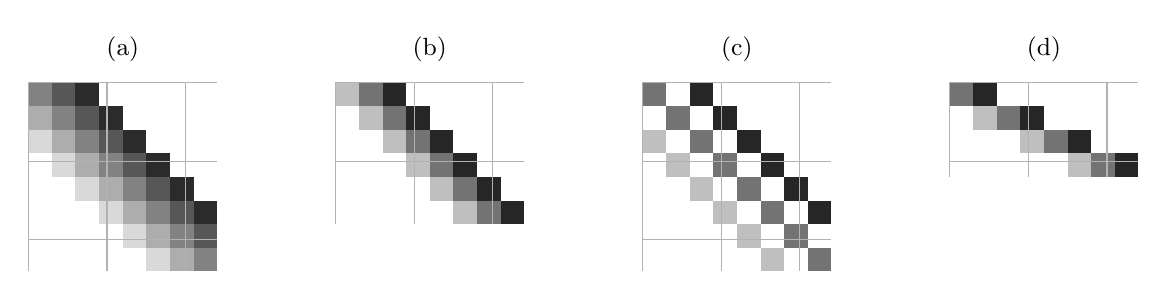
\begin{tikzpicture}[x=0.3cm, y=0.3cm]
    % (a) kernel 5, stride 1, dilation 1, zero padding: 8 rows
    \begin{scope}
      \foreach \r in {1,...,8} {
        \foreach \j in {1,...,5} {
          \pgfmathtruncatemacro{\c}{\r+\j-3}
          \pgfmathtruncatemacro{\s}{15+17*(\j-1)}
          \ifnum\c>0 \ifnum\c<9
            \fill[black!\s] (\c-1,-\r) rectangle ++(1,1);
          \fi\fi
        }
      }
      \draw[gray!60] (0,-8) grid (8,0);
      \node[font=\small] at (4,1.4) {(a)};
    \end{scope}
    % (b) kernel 3, stride 1, dilation 1, valid: 6 rows
    \begin{scope}[xshift=3.9cm]
      \foreach \r in {1,...,6} {
        \foreach \j in {1,2,3} {
          \pgfmathtruncatemacro{\c}{\r+\j-1}
          \pgfmathtruncatemacro{\s}{25+30*(\j-1)}
          \fill[black!\s] (\c-1,-\r) rectangle ++(1,1);
        }
      }
      \draw[gray!60] (0,-6) grid (8,0);
      \node[font=\small] at (4,1.4) {(b)};
    \end{scope}
    % (c) kernel 3, stride 1, dilation 2, zero padding: 8 rows
    \begin{scope}[xshift=7.8cm]
      \foreach \r in {1,...,8} {
        \foreach \j in {1,2,3} {
          \pgfmathtruncatemacro{\c}{\r+2*(\j-2)}
          \pgfmathtruncatemacro{\s}{25+30*(\j-1)}
          \ifnum\c>0 \ifnum\c<9
            \fill[black!\s] (\c-1,-\r) rectangle ++(1,1);
          \fi\fi
        }
      }
      \draw[gray!60] (0,-8) grid (8,0);
      \node[font=\small] at (4,1.4) {(c)};
    \end{scope}
    % (d) kernel 3, stride 2, dilation 1, zero padding: 4 rows
    \begin{scope}[xshift=11.7cm]
      \foreach \r in {1,...,4} {
        \foreach \j in {1,2,3} {
          \pgfmathtruncatemacro{\c}{2*\r-1+\j-2}
          \pgfmathtruncatemacro{\s}{25+30*(\j-1)}
          \ifnum\c>0 \ifnum\c<9
            \fill[black!\s] (\c-1,-\r) rectangle ++(1,1);
          \fi\fi
        }
      }
      \draw[gray!60] (0,-4) grid (8,0);
      \node[font=\small] at (4,1.4) {(d)};
    \end{scope}
  \end{tikzpicture}
  \caption{Weight matrices $\Omega$ of four one-dimensional convolutional layers
  with eight inputs (columns) and one row per output; shading marks the kernel
  weights $\omega_1,\omega_2,\dots$ from light to dark, white entries are zero.
  (a) Kernel size 5, stride 1, dilation 1, zero padding. (b) Kernel size 3,
  stride 1, dilation 1, valid (six outputs). (c) Kernel size 3, stride 1,
  dilation 2, zero padding. (d) Kernel size 3, stride 2, dilation 1, zero padding
  (four outputs).}
  \label{fig:conv-matrices}
\end{figure}

\noindent
The same reading works on a connectivity diagram in which every output is drawn
with lines to its inputs: count the lines entering one output (kernel size),
check how far the pattern moves between neighboring outputs (stride), check
whether the connected inputs are adjacent or spaced (dilation), and compare the
number of outputs with the number of inputs (padding or valid). In
Figure~\ref{fig:conv-matrices}(c), for example, $h_1$ is connected to $x_1$ and
$x_3$ only, because its left tap would need $x_{-1}$; the missing tap is the
signature of zero padding, and the gap of one position between taps is the
signature of dilation $2$.

\subsection{Channels, Receptive Fields, and Why Convolution Helps}

One kernel per layer is not enough, and one layer is not enough either. The
layer is first widened with channels, then the network is deepened until its
units see large parts of the input, and finally the complete design is tested
against a fully connected network.

A single convolution followed by ReLU averages its inputs and then discards all
negative responses, so one such output necessarily loses information about the
input. The remedy is to apply \emph{several} convolutions with different kernels
in parallel and to keep all their outputs. Each output signal is a
\emph{channel}, also called a \emph{feature map}. With two kernels, one might
respond to rising and the other to falling intensity; together they keep what a
single one would lose.

The next layer then receives a multi-channel input, and its kernels must span all
input channels. A kernel for an input with $C_i$ channels has size $C_i\times K$:
it takes a weighted sum over $K$ neighboring positions \emph{and} over all
$C_i$ channels, and produces one output channel. A layer with $C_o$ output
channels uses $C_o$ such kernels, so its weights form a tensor
$\Omega\in\mathbb{R}^{C_i\times C_o\times K}$ and its biases a vector
$\beta\in\mathbb{R}^{C_o}$. For a multi-channel input $X \in
\mathbb{R}^{D\times C_i}$ the output of channel $k$ at position $i$ is
\begin{equation}
  h_{i}^{(k)} = a\Bigl[\beta_k
    + \sum_{c=1}^{C_i}\sum_{j=1}^{K} \omega_{c,k,j}\; x_{i+j-2}^{(c)}\Bigr].
\end{equation}
\noindent
Every output position therefore sees a small neighborhood of the input in
\emph{all} channels. In two dimensions this is the familiar picture: an input
tensor of size $H\times W\times C$ is mapped to an output of size
$H\times W\times C_o$ (with same padding), one feature map per kernel.

The parameter counts follow directly from the tensor shapes
(Table~\ref{tab:conv-params}). One output channel of a one-dimensional layer
needs $C_i K$ weights and one bias; $C_o$ output channels need $C_i C_o K$
weights and $C_o$ biases. None of these numbers depends on the length of the
input.

\begin{table}[ht]
  \centering
  \begin{tabular}{@{}lll@{}}
    \toprule
    Layer & Weights & Biases \\
    \midrule
    1D convolution, $C_i$ inputs, one output channel & $C_i K$ & $1$ \\
    1D convolution, $C_i \rightarrow C_o$ channels & $C_i C_o K$ & $C_o$ \\
    2D convolution, $K\times K$ kernel, $C_i \rightarrow C_o$ &
      $C_i C_o K^2$ & $C_o$ \\
    $1\times1$ convolution, $C_i \rightarrow C_o$ & $C_i C_o$ & $C_o$ \\
    Fully connected, $D_i \rightarrow D_o$ units & $D_i D_o$ & $D_o$ \\
    \bottomrule
  \end{tabular}
  \caption{Parameter counts of convolutional and fully connected layers. The
  convolutional counts are independent of the spatial size of the input.}
  \label{tab:conv-params}
\end{table}

\noindent
Two quick examples fix the formulas. A $3\times3$ convolution from an RGB image
($C_i = 3$) to $C_o = 64$ feature maps has $3\cdot64\cdot9 + 64 = 1{,}792$
parameters, whether the image has $32\times32$ or $1000\times1000$ pixels. A
fully connected layer between the same $224\times224\times3$ input and a
$224\times224\times64$ output would need about $150{,}528\cdot3.2\cdot10^6
\approx 4.8\cdot10^{11}$ weights. The difference of more than eight orders of
magnitude is the whole point of convolution.

Channels widen what a layer computes at one position; depth widens how much of
the input a unit sees. A hidden unit in the first layer sees $K$ inputs. A unit in the second layer sees
$K$ units of the first layer, each of which sees $K$ inputs, so the region of
the input that can influence it has grown. The \emph{receptive field} of a unit is
this region: the set of input positions that can change its value.
Figure~\ref{fig:receptive-field} shows the growth for kernel size $3$ and stride
$1$: the receptive field is $3$ after one layer, $5$ after two, $7$ after three,
and in general $2L+1$ after $L$ layers.

\begin{figure}[ht]
  \centering
  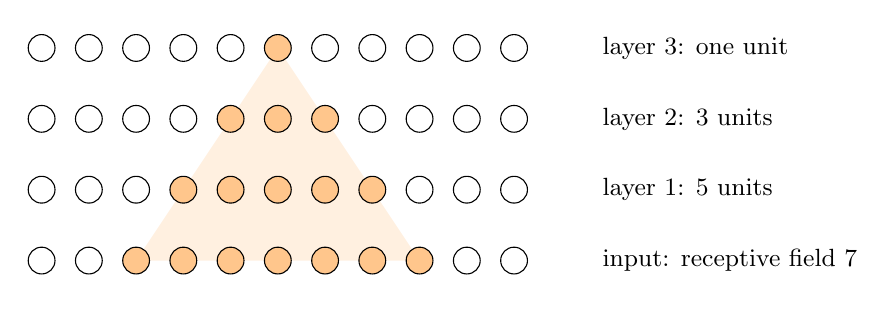
\begin{tikzpicture}[
      unit/.style={circle, draw, minimum size=0.34cm, inner sep=0pt},
      on/.style={unit, fill=orange!45}
    ]
    \fill[orange!12] (2*0.6,0) -- (8*0.6,0) -- (5*0.6,3*0.9) -- cycle;
    \foreach \l/\lo/\hi in {0/2/8, 1/3/7, 2/4/6, 3/5/5} {
      \foreach \i in {0,...,10} {
        \pgfmathtruncatemacro{\inside}{(\i>=\lo) && (\i<=\hi)}
        \ifnum\inside=1
          \node[on] at (0.6*\i,0.9*\l) {};
        \else
          \node[unit] at (0.6*\i,0.9*\l) {};
        \fi
      }
    }
    \node[anchor=west, font=\small] at (7.0,0) {input: receptive field $7$};
    \node[anchor=west, font=\small] at (7.0,0.9) {layer 1: $5$ units};
    \node[anchor=west, font=\small] at (7.0,1.8) {layer 2: $3$ units};
    \node[anchor=west, font=\small] at (7.0,2.7) {layer 3: one unit};
  \end{tikzpicture}
  \caption{Receptive field of one unit in the third layer of a network with
  kernel size 3 and stride 1. Each layer adds $K-1=2$ positions, so the unit
  depends on seven input values.}
  \label{fig:receptive-field}
\end{figure}

\noindent
Stride and dilation make the growth much faster. After a layer with stride $S$,
neighboring units are $S$ input positions apart, so every later kernel tap
reaches $S$ times further. Let $r_l$ be the receptive field after layer $l$ and
$j_l$ the distance, measured in input positions, between neighboring units of
layer $l$ (with $r_0 = 1$, $j_0 = 1$). Then
\begin{equation}
  r_l = r_{l-1} + \bigl(K_{\mathrm{eff},l} - 1\bigr)\, j_{l-1},
  \qquad
  j_l = j_{l-1}\, S_l .
  \label{eq:receptive-field}
\end{equation}
\noindent
For three layers with kernel size $3$ and stride $2$ this gives
$r = 3, 7, 15$ with $j = 2, 4, 8$: the receptive field roughly doubles per layer
instead of growing by two. Pooling layers count like convolutions in this
recursion, with their window size as $K$.

Growing receptive fields are why depth matters for images. Early units see a few
pixels and can only respond to local patterns such as edges and color blobs.
Units a few layers deeper combine these into corners, textures, and repeated
motifs; the deepest units see large parts of the image and respond to object
parts and whole objects. Resolution, kernel size, stride, and pooling together
decide which spatial scale a layer can capture. A useful side effect concerns
kernel size: two stacked $3\times3$ layers have the same $5\times5$ receptive
field as one $5\times5$ layer, but need $2\cdot9\,C^2 = 18C^2$ instead of $25C^2$
weights for $C$ channels, and they add a second nonlinearity. This is the design
principle of the VGG network discussed below.

\paragraph{Putting it together: MNIST-1D.}
How much does the convolutional structure actually help? MNIST-1D is a small
benchmark built for this question. Each of ten digit templates is a
one-dimensional curve; a training example is a randomly transformed template
with added noise, sampled at $40$ positions. The class does not depend on where
along the signal the pattern appears, which is exactly the kind of structure a
convolutional network is designed for.

The convolutional network for this task has three convolutional layers and one fully connected layer,
followed by softmax. All convolutions are valid, with kernel size $3$, stride
$2$, and $15$ channels. The output sizes follow from
Eq.~\eqref{eq:conv-outsize}, and the parameter counts from
Table~\ref{tab:conv-params}:
\begin{center}
  \begin{tabular}{@{}lccr@{}}
    \toprule
    Layer & Output size & Computation & Parameters \\
    \midrule
    input & $40\times1$ & & \\
    conv 1 ($1\rightarrow15$) & $19\times15$ &
      $\lfloor 37/2\rfloor+1 = 19$ & $1\cdot15\cdot3+15 = 60$ \\
    conv 2 ($15\rightarrow15$) & $9\times15$ &
      $\lfloor 16/2\rfloor+1 = 9$ & $15\cdot15\cdot3+15 = 690$ \\
    conv 3 ($15\rightarrow15$) & $4\times15$ &
      $\lfloor 6/2\rfloor+1 = 4$ & $690$ \\
    fully connected ($60\rightarrow10$) & $10$ & $4\cdot15 = 60$ inputs &
      $60\cdot10+10 = 610$ \\
    \midrule
    total & & & $2{,}050$ \\
    \bottomrule
  \end{tabular}
\end{center}
\noindent
By Eq.~\eqref{eq:receptive-field}, the units of the three convolutional layers
have receptive fields of $3$, $7$, and $15$ input samples; the fully connected
layer then combines all of them. The network is trained with SGD for $100{,}000$
steps with learning rate $0.01$ and batch size $100$.

For comparison, a fully connected network with exactly the same number of layers and hidden
units has $150{,}185$ parameters, more than seventy times as many. Its training
error drops to zero within a small fraction of the training steps, but its test
error stays at roughly $40\%$. The convolutional network fits the training data
more slowly and still reaches a test error of only about $17\%$. The fully
connected network overfits (Section~\ref{sec:neural-networks}): it has enough
freedom to memorize the training set and nothing that guides it toward rules
that transfer to new examples.

The reason is the \emph{inductive bias} of convolution, the prior assumption
built into the architecture. The convolutional network is forced to process
every position in the same way, so what it learns from a pattern at one position
is immediately available at all other positions: information is shared across
locations. It searches through a much smaller family of input--output mappings,
and all members of that family are plausible for signals in which position does
not matter. A fully connected network could in principle represent the same
function, but it would have to discover weight sharing from data alone.

\subsection{Convolutional Networks for Image Classification}

Images are two-dimensional, and the convolutional layer extends to them without
new ideas. The kernel becomes a $K\times K$ grid of weights, and each output is a
weighted sum over a $K\times K$ neighborhood, plus a bias, passed through the
activation:
\begin{equation}
  h_{ij} = a\Bigl[\beta + \sum_{m=1}^{K}\sum_{n=1}^{K}
    \omega_{mn}\; x_{i+m-\lceil K/2\rceil,\; j+n-\lceil K/2\rceil}\Bigr].
\end{equation}
\noindent
With $C_i$ input channels the kernel has size $C_i\times K\times K$ and the sum
also runs over the channels; $C_o$ such kernels produce $C_o$ output channels
with $C_i C_o K^2$ weights and $C_o$ biases (Table~\ref{tab:conv-params}).
Stride, dilation, and padding act separately along the rows and the columns,
and Eq.~\eqref{eq:conv-outsize} gives the output height and width.

\paragraph{Downsampling.}
Classification networks gradually reduce the spatial resolution. This saves
computation, enlarges the receptive fields of later layers, and aggregates
evidence over larger regions. Three standard operations halve the resolution
of a feature map:
\begin{itemize}
  \item \emph{subsampling}: keep every other position in each direction, which
        is equivalent to a convolution with stride $2$;
  \item \emph{max pooling}: keep the maximum of each $2\times2$ block; small
        shifts of a feature inside a block do not change the result, which gives
        partial invariance to translation;
  \item \emph{mean pooling}: keep the average of each $2\times2$ block.
\end{itemize}
\noindent
Pooling acts on each channel separately and has no parameters. For the
$4\times4$ feature map below, split into four $2\times2$ blocks,
\begin{equation*}
  \begin{pmatrix}
    1 & 3 & 2 & 0\\ 4 & 2 & 1 & 1\\ 0 & 1 & 5 & 6\\ 2 & 0 & 7 & 8
  \end{pmatrix}
  \;\xrightarrow{\ \text{max}\ }\;
  \begin{pmatrix} 4 & 2\\ 2 & 8 \end{pmatrix},
  \qquad
  \xrightarrow{\ \text{mean}\ }\;
  \begin{pmatrix} 2.5 & 1\\ 0.75 & 6.5 \end{pmatrix},
  \qquad
  \xrightarrow{\ \text{subsample}\ }\;
  \begin{pmatrix} 1 & 2\\ 0 & 5 \end{pmatrix}.
\end{equation*}
\noindent
In the backward pass, max pooling behaves like the maximum node of
Table~\ref{tab:gate-rules}: the gradient is routed only to the position that
held the maximum. Mean pooling distributes it equally over the block.

Networks that must output an image-sized result, such as a segmentation, need the
reverse operation. The simplest is to \emph{duplicate} every value into a
$2\times2$ block. \emph{Max-upsampling} (max-unpooling) remembers where each
maximum came from during max pooling and writes the value back to exactly that
position, filling the rest with zeros. \emph{Bilinear interpolation} fills the
new positions with weighted averages of their neighbors. A learned alternative is
the transposed convolution, which spreads each input value over a neighborhood
with learned weights.

A last special case is the $1\times1$ convolution. A kernel of spatial size $1\times1$ looks at a single position but at all $C_i$
channels. It computes, at every pixel independently, a weighted combination of
the channels. This is equivalent to running the same small fully connected
network at every position. It mixes information between channels and changes
their number, from $C_i$ to $C_o$, at the cost of only $C_i C_o + C_o$
parameters. It is often used to reduce the number of channels before an
expensive $3\times3$ layer.

\paragraph{Image classification and the ConvNet layout.}
With these building blocks, full image classifiers can be assembled. Image
classification is a multiclass problem: the network receives an image and
outputs a probability for each of more than two discrete classes. Deep networks
won this task on the ImageNet benchmark, a database of millions of labeled
images in $1{,}000$ classes, typically resized to $224\times224$ pixels. Results
are reported as \emph{top-1 error} (the highest-scoring class is wrong) and
\emph{top-5 error} (the correct class is not among the five highest-scoring
ones).

Almost every classification network follows the layout of
Figure~\ref{fig:convnet-layout}. A stack of blocks, each made of convolution and
ReLU, often followed by max pooling, reduces the resolution step by step while
increasing the number of channels: spatial detail is traded for more abstract
features. At the end, the feature maps are flattened (or averaged over all
positions) into one vector, and one or more fully connected layers followed by a
softmax produce the class probabilities. Training minimizes the cross-entropy
loss with SGD and backpropagation exactly as in
Section~\ref{sec:neural-networks}. ReLU is the standard activation function in
ConvNets because it is cheap and does not saturate for positive inputs.

\begin{figure}[ht]
  \centering
  \begin{tikzpicture}[
      node distance=0.42cm,
      box/.style={draw, rounded corners, align=center, font=\small,
        minimum height=1.1cm, text width=1.75cm},
      arrow/.style={-{Latex[length=2mm]}, thick}
    ]
    \node[box, fill=green!8] (img) {image\\$224{\times}224{\times}3$};
    \node[box, fill=blue!8, right=of img] (c1) {conv + ReLU\\max pool};
    \node[box, fill=blue!8, right=of c1] (c2) {conv + ReLU\\max pool};
    \node[font=\small, right=0.25cm of c2] (dots) {$\cdots$};
    \node[box, fill=orange!12, right=0.25cm of dots] (fc) {flatten\\fully conn.};
    \node[box, fill=red!8, right=of fc] (sm) {softmax\\class prob.};
    \draw[arrow] (img) -- (c1);
    \draw[arrow] (c1) -- (c2);
    \draw[arrow] (fc) -- (sm);
    \draw[decorate, decoration={brace, amplitude=5pt, mirror}, thick]
      ([yshift=-0.2cm]c1.south west) -- ([yshift=-0.2cm]dots.south east)
      node[midway, below=0.25cm, font=\small, align=center]
      {feature extraction: resolution $\downarrow$, channels $\uparrow$};
    \draw[decorate, decoration={brace, amplitude=5pt, mirror}, thick]
      ([yshift=-0.2cm]fc.south west) -- ([yshift=-0.2cm]sm.south east)
      node[midway, below=0.25cm, font=\small] {classifier};
  \end{tikzpicture}
  \caption{Basic layout of a convolutional network for classification.
  Convolution--ReLU--pooling blocks extract increasingly abstract features at
  decreasing resolution; fully connected layers and a softmax turn them into
  class probabilities.}
  \label{fig:convnet-layout}
\end{figure}

\paragraph{AlexNet (2012).}
AlexNet was the first convolutional network to win ImageNet, by a large margin.
It has five convolutional layers, some followed by max pooling, and three fully
connected layers, with ReLU activations throughout. Of its roughly $60$ million
parameters, almost all sit in the fully connected layers; the convolutional
layers are cheap by Table~\ref{tab:conv-params}. Such a model overfits easily,
and AlexNet introduced or popularized the regularization tools that are still
standard (Section~\ref{sec:neural-networks}):
\begin{itemize}
  \item \emph{Data augmentation} enlarged the training set by a factor of $2048$,
        using spatial transformations (random crops and horizontal mirroring)
        and modifications of the input intensities. The network sees a
        slightly different version of every image in every epoch, and it must
        give all of them the same label.
  \item \emph{Dropout} in the fully connected layers sets the output of a random
        subset of neurons to zero, only during training. No unit can rely on
        a particular other unit being present, which reduces overfitting; at test
        time all units are used.
  \item \emph{Test-time averaging}: the prediction is the average over five
        crops of the image and their mirrored versions, a form of augmentation
        at test time.
  \item SGD with momentum $0.9$, batch size $128$, and an $L_2$ weight-decay
        penalty on large weights.
\end{itemize}
\noindent
AlexNet reached a top-5 error of $16.4\%$ and a top-1 error of $38.1\%$.

\paragraph{VGG (2015).}
The VGG networks pushed depth further with a deliberately simple design: only
$3\times3$ convolutions (stride $1$, same padding) and $2\times2$ max pooling,
with the number of channels doubling after each pooling step. As shown above for
receptive fields, stacks of small kernels reach large receptive
fields with fewer weights and more nonlinearities than one large kernel. The
largest variant has $19$ weight layers and $144$ million parameters and reached
a top-5 error of $6.8\%$ and a top-1 error of $23.7\%$.
Table~\ref{tab:alexnet-vgg} compares the two networks. Over the following years
the ImageNet error kept falling as networks grew deeper, until residual
networks made training of very deep networks routine and
surpassed human-level top-5 performance.

\begin{table}[ht]
  \centering
  \begin{tabular}{@{}p{3.4cm}p{5.0cm}p{5.0cm}@{}}
    \toprule
    & AlexNet (2012) & VGG-19 (2015) \\
    \midrule
    Depth & 5 convolutional + 3 fully connected & 16 convolutional + 3 fully
      connected \\
    Kernels & large in the first layer, then smaller & $3\times3$ everywhere \\
    Parameters & about 60 million, mostly fully connected & 144 million \\
    Regularization & augmentation, dropout, weight decay & augmentation, dropout,
      weight decay \\
    Top-5 / top-1 error & $16.4\%$ / $38.1\%$ & $6.8\%$ / $23.7\%$ \\
    \bottomrule
  \end{tabular}
  \caption{Two landmark ImageNet classifiers. VGG replaces large kernels by deep
  stacks of $3\times3$ convolutions and roughly halves the error.}
  \label{tab:alexnet-vgg}
\end{table}

\paragraph{Pre-training and fine-tuning.}
Networks of this size need millions of labeled images, which most applications
do not have. \emph{Pre-training} solves this by \emph{transfer learning}. The
network is first trained on a large dataset such as ImageNet. Its early layers
then contain generic feature detectors (edges, color blobs, textures, simple
parts) that are useful for almost any image task. For the new task, the final
classification layer is replaced by a new one with the right number of classes.
With little data, the pre-trained layers are \emph{frozen} and only the new head
is trained, so the network acts as a fixed feature extractor. With more data,
all layers are \emph{fine-tuned} with a small learning rate, starting from the
pre-trained weights instead of a random initialization. Either way the network
starts from a good representation and needs far fewer labeled examples than
training from scratch.

\subsection{Object Detection and Semantic Segmentation}

Classification produces one label for the whole image. Many applications need
more: \emph{where} the objects are, and which pixels belong to them. Both tasks
reuse the convolutional building blocks, but change what the network outputs.

\paragraph{Object detection with YOLO.}
An object detector outputs a set of bounding boxes, each with a class. YOLO
(``You Only Look Once'') does this with a single forward pass of a network
similar to VGG, applied to a $448\times448$ input. The final feature map is
interpreted as a $7\times7$ grid of cells over the image
(Figure~\ref{fig:yolo}). Each cell predicts
\begin{itemize}
  \item class probabilities for the object whose center falls into the cell, and
  \item two bounding boxes, each described by five numbers: the center $(x,y)$,
        the width and height, and a confidence that the box contains an object.
\end{itemize}
\noindent
For $C$ classes the output therefore has $7\times7\times(2\cdot5 + C)$ entries;
with the $C = 20$ classes of the PASCAL VOC dataset this is
$7\cdot7\cdot30 = 1{,}470$ numbers. All $98$ candidate boxes are produced at
once, which is what makes YOLO fast. A heuristic at the end discards boxes with
low confidence and removes duplicates that overlap strongly with a more
confident box of the same class (non-maximum suppression). Training uses the
same toolbox as for classification: momentum, weight decay, dropout, and data
augmentation.

\begin{figure}[ht]
  \centering
  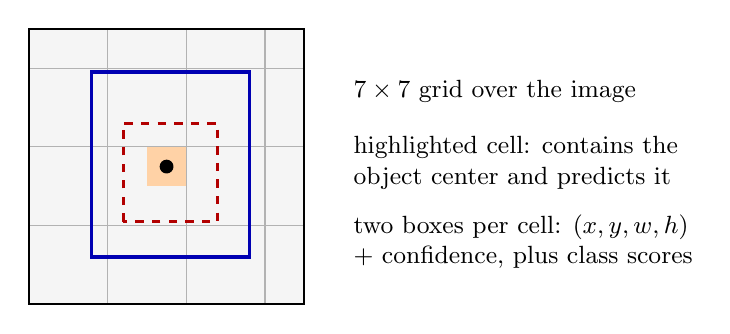
\begin{tikzpicture}[x=0.5cm, y=0.5cm]
    \fill[gray!8] (0,0) rectangle (7,7);
    \fill[orange!35] (3,3) rectangle (4,4);
    \draw[gray!60] (0,0) grid (7,7);
    \draw[thick] (0,0) rectangle (7,7);
    \draw[very thick, blue!70!black] (1.6,1.2) rectangle (5.6,5.9);
    \draw[very thick, red!70!black, dashed] (2.4,2.1) rectangle (4.8,4.6);
    \fill (3.5,3.5) circle (2.5pt);
    \node[anchor=west, font=\small, align=left] at (8,5.4)
      {$7\times7$ grid over the image};
    \node[anchor=west, font=\small, align=left] at (8,3.6)
      {highlighted cell: contains the\\object center and predicts it};
    \node[anchor=west, font=\small, align=left] at (8,1.6)
      {two boxes per cell: $(x,y,w,h)$\\+ confidence, plus class scores};
  \end{tikzpicture}
  \caption{YOLO divides the image into a $7\times7$ grid. The cell containing an
  object's center predicts class scores and two candidate boxes (solid and
  dashed); a final thresholding step keeps the confident, non-duplicate boxes.}
  \label{fig:yolo}
\end{figure}

\paragraph{Semantic segmentation.}
\emph{Semantic segmentation} assigns a class label to every pixel of the image,
for example road, car, pedestrian, or background. It does not distinguish
between two objects of the same class; all car pixels simply receive the label
``car''. Formally it is a multivariate classification problem: one output per
pixel, each a binary (object versus background) or multiclass decision. The
output must be as large as the input and, by the argument on invariance and
equivariance, should move with the image content.

The standard solution is a convolutional \emph{encoder--decoder} network
(Figure~\ref{fig:encoder-decoder}). The \emph{encoder} is a classification-style
network, for example the convolutional part of VGG: it reduces the resolution
and builds features with large receptive fields that know \emph{what} is in the
image. The \emph{decoder} mirrors it with upsampling layers (for example
max-unpooling at the positions stored by the encoder's max pooling) and
convolutions, recovering \emph{where} each class lies at full resolution. The
final layer is a $1\times1$ convolution with one channel per class and a softmax
at every pixel, and the loss is the sum of the per-pixel cross-entropies.
Because every layer is convolutional, the whole network is equivariant, and the
per-pixel classifier shares its weights across the image. The U-Nets of later
sections improve this design by adding skip connections that pass fine details
from the encoder directly to the decoder.

\begin{figure}[ht]
  \centering
  \begin{tikzpicture}[
      blk/.style={draw, fill=blue!10, minimum width=0.45cm},
      arrow/.style={-{Latex[length=2mm]}, thick}
    ]
    \node[draw, fill=green!8, minimum width=0.35cm, minimum height=2.6cm]
      (in) at (0,0) {};
    \node[blk, minimum height=2.6cm] (e1) at (1.3,0) {};
    \node[blk, minimum height=1.8cm] (e2) at (2.5,0) {};
    \node[blk, minimum height=1.1cm] (e3) at (3.7,0) {};
    \node[draw, fill=orange!25, minimum width=0.45cm, minimum height=0.6cm]
      (b) at (4.9,0) {};
    \node[blk, minimum height=1.1cm] (d3) at (6.1,0) {};
    \node[blk, minimum height=1.8cm] (d2) at (7.3,0) {};
    \node[blk, minimum height=2.6cm] (d1) at (8.5,0) {};
    \node[draw, fill=red!10, minimum width=0.35cm, minimum height=2.6cm]
      (out) at (9.8,0) {};
    \foreach \a/\b in {in/e1, e1/e2, e2/e3, e3/b, b/d3, d3/d2, d2/d1, d1/out} {
      \draw[arrow] (\a) -- (\b);
    }
    \node[above=0.15cm of in, font=\small] {image};
    \node[above=0.15cm of out, font=\small] {label map};
    \node[above=0.15cm of b, font=\small, align=center] {bottleneck};
    \draw[decorate, decoration={brace, amplitude=5pt, mirror}, thick]
      (1.05,-1.55) -- (3.95,-1.55)
      node[midway, below=0.25cm, font=\small, align=center]
      {encoder: conv + pooling\\resolution $\downarrow$};
    \draw[decorate, decoration={brace, amplitude=5pt, mirror}, thick]
      (5.85,-1.55) -- (8.75,-1.55)
      node[midway, below=0.25cm, font=\small, align=center]
      {decoder: upsampling + conv\\resolution $\uparrow$};
  \end{tikzpicture}
  \caption{Convolutional encoder--decoder for semantic segmentation. Box heights
  indicate spatial resolution. The encoder compresses the image into features
  with large receptive fields; the decoder upsamples them back to one class
  distribution per pixel.}
  \label{fig:encoder-decoder}
\end{figure}

\noindent
Table~\ref{tab:cnn-tasks} summarizes how the three tasks differ in their output
and in the network that produces it.

\begin{table}[ht]
  \centering
  \begin{tabular}{@{}p{2.8cm}p{3.7cm}p{3.4cm}p{3.6cm}@{}}
    \toprule
    Task & Output & Desired property & Network \\
    \midrule
    Classification & one class distribution per image & translation invariance &
      conv--pool stack, fully connected layers, softmax \\
    Object detection & boxes with class and confidence & box positions move with
      the objects & conv backbone with a grid of box predictions (YOLO) \\
    Semantic segmentation & one class per pixel & translation equivariance &
      encoder--decoder, per-pixel softmax \\
    \bottomrule
  \end{tabular}
  \caption{Three visual tasks solved with convolutional networks. They share the
  convolutional feature extractor and differ in the output layer and in whether
  spatial position is discarded or kept.}
  \label{tab:cnn-tasks}
\end{table}
